\documentclass[11pt]{article}
\usepackage[utf8]{vietnam}
\usepackage{hyperref}
\usepackage{makecell}
\usepackage{blindtext}
\usepackage{xcolor}
\usepackage{enumitem}
\usepackage{listings}
\hypersetup{
    colorlinks=true, 
    linkcolor=blue,
    filecolor=magenta,      
    urlcolor=red,
    pdftitle={Overleaf Example},
    pdfpagemode=FullScreen,
    }
\usepackage{amsmath,amssymb,amsfonts}
\usepackage{graphicx}

\setlength{\topmargin}{-.5in} \setlength{\textheight}{9.25in}
\setlength{\oddsidemargin}{0in} \setlength{\textwidth}{6.8in}

%%%%%%%%%%%%%%%%%%%%%%%%%%%%%%%%%%%%%%%%%%
% \usepackage{pythonhighlight}
%%%%%%%%%%%%%%%%%%%%%%%%%%%
\newcounter{mycounter} % create a new counter, called 'mycounter'
% default def'n of '\themycounter' is '\arabic{mycounter}'
%% command to increment 'mycounter' by 1 and to display its value:
\newcommand\showmycounter{\stepcounter{mycounter}\themycounter}
\usepackage{lipsum}
\newcommand\showlips{\stepcounter{mycounter}\lipsum[\value{mycounter}]}
%%%%%%%%%%%%%%%%%%%%%%%%%%%%%%%%%%%%%%
\usepackage{framed}
\usepackage{hyperref}
\usepackage{fancyhdr}

%%%%%%%%%%%%%%%%%%%%%%%%%%%%%%%%%%%%%%%%%%%%%%%%%%%%%%%%%%%%%
\usepackage{listings}
\usepackage{xcolor}

\definecolor{codegreen}{rgb}{0,0.6,0}
\definecolor{codegray}{rgb}{0.5,0.5,0.5}
\definecolor{codepurple}{rgb}{0.58,0,0.82}
\definecolor{backcolour}{rgb}{0.95,0.95,0.92}

\lstdefinestyle{mystyle}{
    backgroundcolor=\color{backcolour},   
    commentstyle=\color{codegreen},
    keywordstyle=\color{magenta},
    numberstyle=\tiny\color{codegray},
    stringstyle=\color{codepurple},
    basicstyle=\ttfamily\footnotesize,
    breakatwhitespace=false,         
    breaklines=true,                 
    captionpos=b,                    
    keepspaces=true,                 
    numbers=left,                    
    numbersep=5pt,                  
    showspaces=false,                
    showstringspaces=false,
    showtabs=false,                  
    tabsize=2
}

\lstset{style=mystyle}
%%%%%%%%%%%%%%%%%%%%%%%%%%%%%%%%%%%%%%%%%%%%%%%%%%%%%%%%%%%%%
\title{\LARGE AI VIET NAM – COURSE 2024}
\author{\Huge \begin{minipage}{\textwidth}\centering Giới thiệu về Figma \end{minipage}}
\pagestyle{fancy}
\fancyhf{}
\lhead{\bfseries AI VIETNAM}
\rhead{\bfseries  aivietnam.edu.vn}
\begin{document}
\maketitle


\section{Giới thiệu}

Figma là một công cụ thiết kế UI/UX rất mạnh mẽ trên nền tảng web, cho phép người dùng thiết kế, tạo nguyên mẫu (prototype) và cộng tác trong thời gian thực. Figma hoạt động trên trình duyệt web nên có thể sử dụng trên tất cả các hệ điều hành phổ biến như Windows, macOS và Linux. Những tính năng nổi trội của Figma: 
\begin{itemize}
    \item Cộng tác trực tuyến: Cho phép nhiều người cùng làm việc trên một dự án, xem và chỉnh sửa thiết kế trong thời gian thực.
    \item Khả năng tích hợp: Dễ dàng tích hợp với nhiều công cụ khác như Slack, Zeplin, và Trello.
    \item Dễ sử dụng: Giao diện người dùng thân thiện và trực quan, phù hợp cho cả người mới bắt đầu.
    \item Plugin: trang bị rất nhiều plugin mạnh mẽ giúp người dùng nâng cao hiệu suất làm việc.
    \item Hỗ trợ lưu trữ đám mây: Figma sử dụng dịch vụ đám mây để lưu trữ và chỉnh sửa dữ liệu, người dùng không cần lo lắng về vấn đề mất mát dữ liệu trong quá trình phát triển sản phẩm.
\end{itemize}

\section{Hướng dẫn đăng ký và sử dụng Figma}
Đăng ký và sử dụng Figma là rất đơn giản, dưới đây là các bước cơ bản để bắt đầu sử dụng:
\begin{itemize}
    \item Truy cập vào \href{https://www.figma.com/}{trang chủ Figma} và đăng ký tài khoản bằng cách nhấn nút “Get Started for free” trên trang chủ. ta có thể đăng ký (đăng nhập) bằng tài khoản Google hoặc email.
          \begin{figure}[!h]
              \centering
              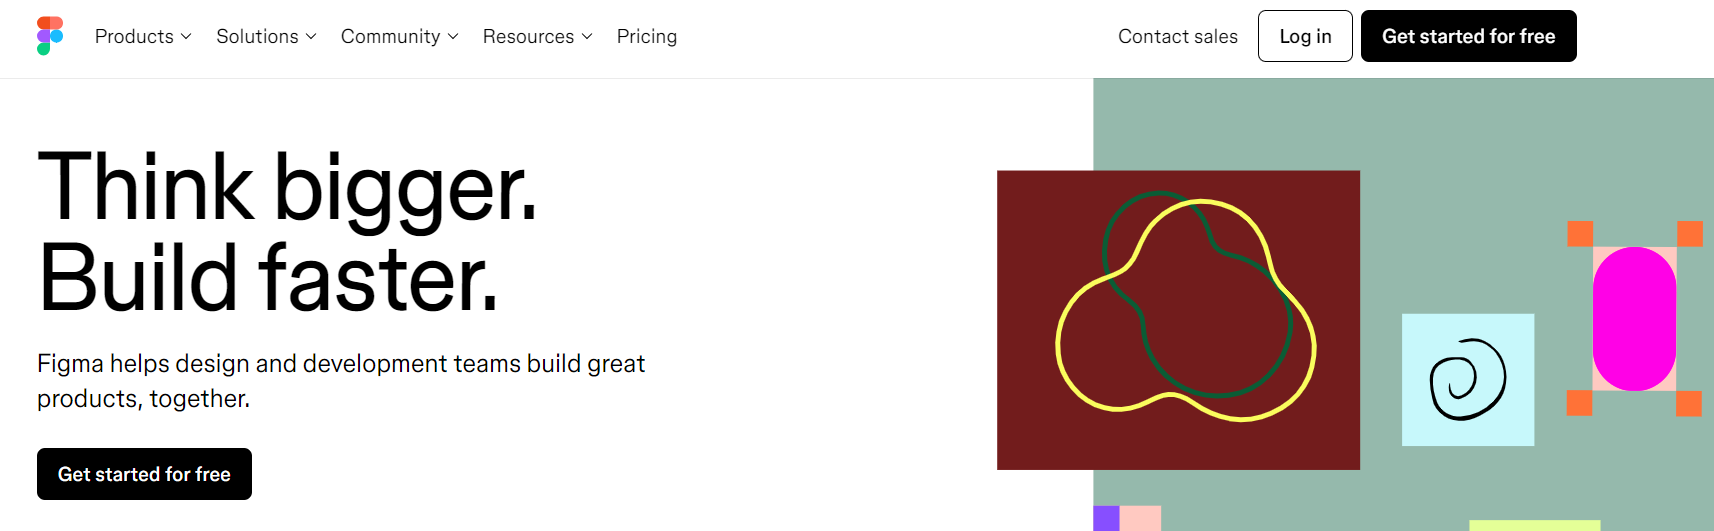
\includegraphics[width=1\linewidth]{imgs/image.png}
              \caption{Màn hình trang chủ Figma}
          \end{figure}
          \newpage
    \item Tiến hành đăng ký/đăng nhập tài khoản. Ta có thể đăng nhập tài khoản có sẵn hoặc cũng có thể tiến hành thông qua tài khoản google bằng cách chọn "Continue with Google" và chọn tài khoản muốn đăng nhập.
          \begin{figure}[!h]
              \centering
              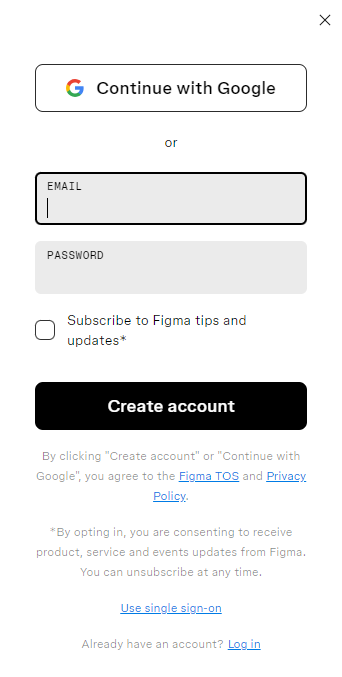
\includegraphics[width=0.5\linewidth]{imgs/image copy.png}
              \caption{Đăng ký/Đăng nhập}
          \end{figure}
          \newpage
    \item Sau khi đăng ký/đăng nhập, ta sẽ được chuyển đến trang quản lý tài khoản. Tại đây, ta có thể thực hiện tạo các bản thiết kế mới hoặc truy cập vào các bản vẽ đã có thông qua các tuỳ chọn trên giao diện. Ta cũng có thể nhập tệp thiết kế đã có sẵn từ máy tính cá nhân bằng cách chọn "Import".

          \begin{figure}[!h]
              \centering
              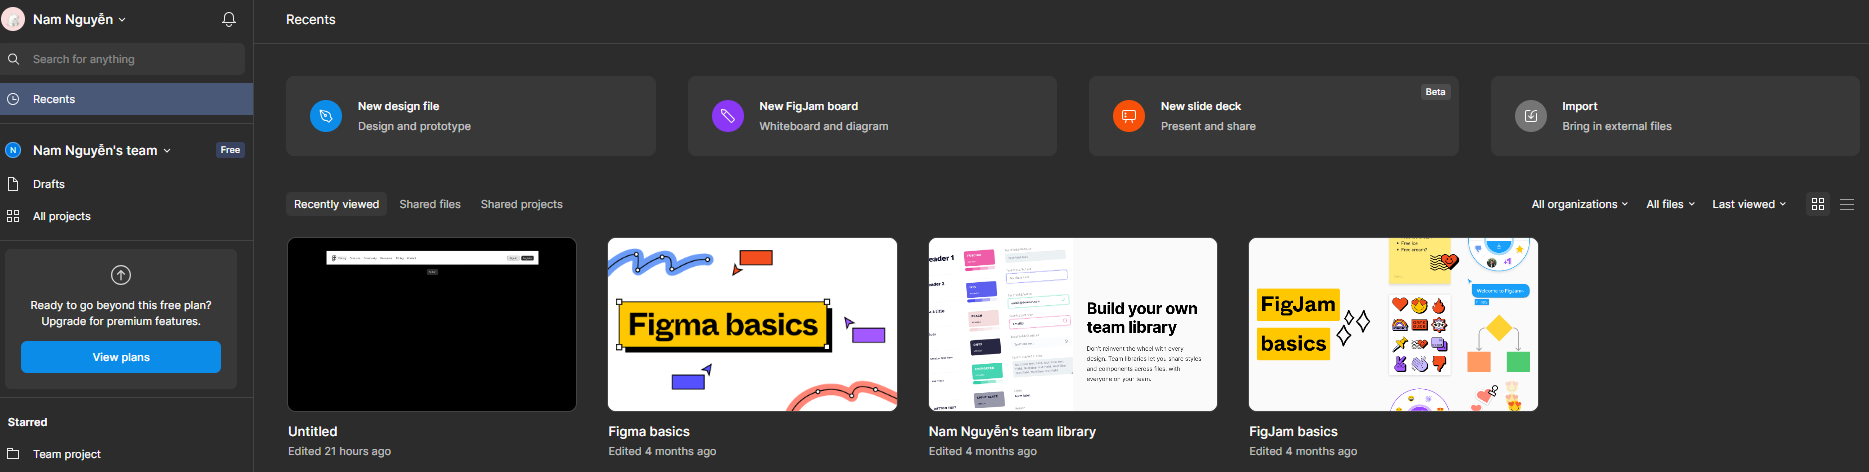
\includegraphics[width=1\linewidth]{imgs/image copy 2.png}
              \caption{Giao diện sau khi Đăng ký/Đăng nhập}
          \end{figure}
\end{itemize}

\section{Các chức năng của Figma}
% \item
%       \textbf{Các chức năng của Figma}

\begin{itemize}
    \item Thiết kế
          \begin{itemize}
              \item Canvas: Khu vực làm việc chính, nơi ta có thể tạo và chỉnh sửa các thành phần thiết kế.
              \item Layers Panel: Quản lý các lớp (layers) của thiết kế, cho phép ta sắp xếp và tổ chức các thành phần.
              \item Assets Panel: Truy cập và quản lý các thành phần tái sử dụng, như biểu tượng (icons) và kiểu chữ (text styles).
              \item Components: Tạo các thành phần dùng chung (components) để tái sử dụng trong nhiều phần của dự án.
              \item Vector Network: Công cụ vẽ vector tiên tiến giúp tạo các hình dạng phức tạp một cách dễ dàng.
              \item Interactions: Tạo các tương tác giữa các khung (frame) để mô phỏng trải nghiệm người dùng.
              \item Animations: Thêm hiệu ứng chuyển động (animation) giữa các khung để làm sinh động thiết kế.
              \item Preview: Xem trước nguyên mẫu trên thiết bị di động hoặc trong trình duyệt để kiểm tra tính khả dụng
          \end{itemize}

    \item Cộng tác
          \begin{itemize}
              \item Real-time Collaboration: Cộng tác với đồng nghiệp trong thời gian thực, nhận phản hồi trực tiếp trên thiết kế, mời và phân quyền thành viên trong dự án.
              \item Comments: Figma cung cấp chức năng bình luận trực tiếp giúp các thành viên trong nhóm dễ dàng trao đổi ý kiến và góp ý nhanh chóng, thuận tiện.
              \item Version History: Figma lưu trữ lịch sử thay đổi của tệp, cho phép xem và khôi phục lại những phiên bản trước đó nếu cần thiết.
              \item Component library: ta có thể tạo và chia sẻ những thành phần dùng chung giữa các dự án, giúp đảm bảo tính nhất quán và tiết kiệm thời gian.
              \item Prototyping (Tạo nguyên mẫu): Figma cho phép tạo nguyên mẫu và chia sẻ cho người khác để thử nghiệm và thu thập phản hồi.
              \item Plugin: Figma hỗ trợ rất nhiều các plugin mạnh mẽ và có thể tích hợp với các công cụ quan lý công việc như: Slack, Jira, Trello,... Các plugin thường sử dụng như: unsplash, anima, iconify,...
          \end{itemize}
\end{itemize}

\section{Hướng dẫn các thao tác với Figma}
% \item
%       \textbf{Hướng dẫn các thao tác với Figma}

\begin{itemize}
    \item Tạo dự án mới: ta tiến hành tạo dự mới bằng cách chọn "New design file".
          \begin{figure}[!h]
              \centering
              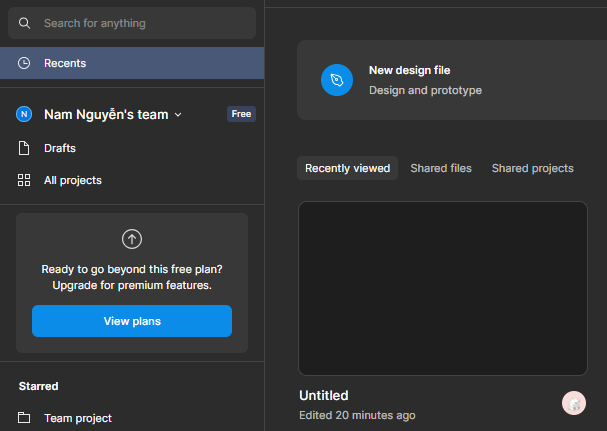
\includegraphics[width=1\linewidth]{imgs/img (1).png}
              \caption{Chọn "New design file" để tạo dự án mới}
          \end{figure}
          \newpage
    \item Giao diện thiết kế sẽ được hiển thị bao gồm: thanh công cụ, khu vực thiết kế, các thành phần (component) và các phím tiện ích khác.

          \begin{figure}[!h]
              \centering
              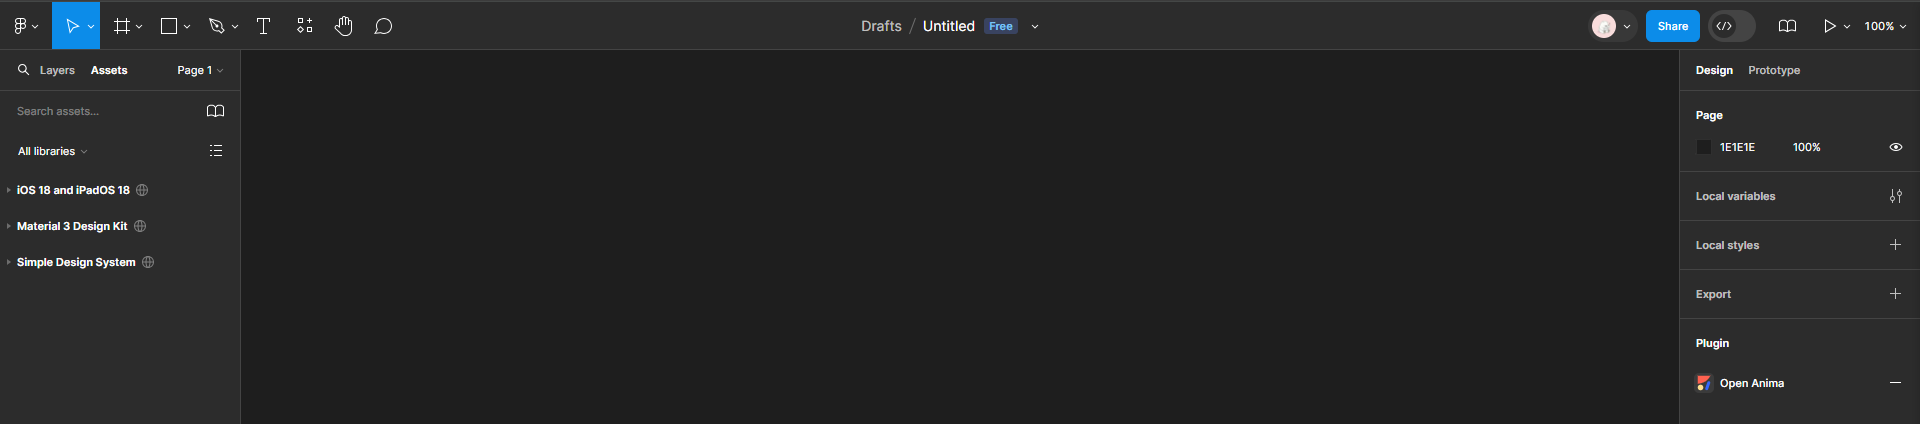
\includegraphics[width=1\linewidth]{imgs/img (2).png}
              \caption{Giao diện Canvas Figma}
          \end{figure}
        


    \item Các công cụ trong Figma:
          % \listoffigures
          \begin{figure}[!h]
              \centering
              
\includegraphics[width=1\linewidth]{imgs/img (3).png}
              \caption{Các công cụ}
          \end{figure}
          \newpage
    \item Move tools: công cụ giúp di chuyển các đối tượng (frame, component,...), ta có thể kéo thả (phím tắt V) hay phóng to/thu nhỏ, thay đổi tỷ lệ của đối tượng (K)
          \begin{figure}[!h]
              \centering
              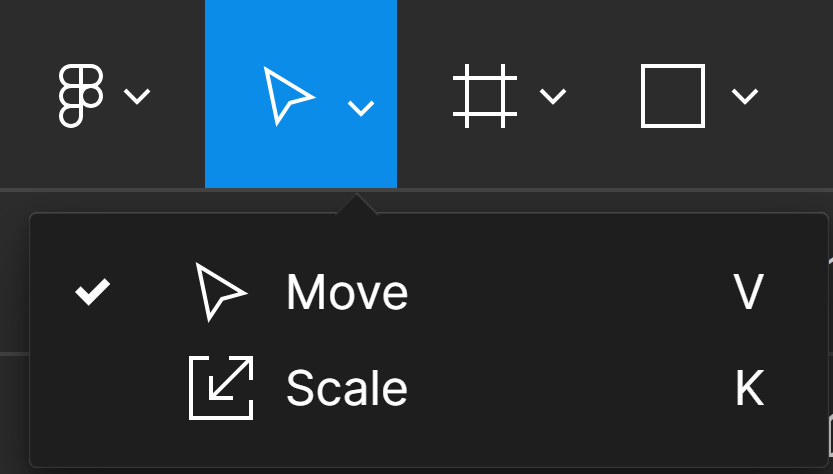
\includegraphics[width=0.5\linewidth]{imgs/img (4).png}
              \caption{Move tools}
          \end{figure}
    \item Region tools: công cụ giúp tạo các đối tượng như  Frame (F): để tạo các khung màn hình khác nhau; Section (Shift+S): tạo các phần để quản lý dễ dàng hơn; Slice(S): để cắt các thành phần của đối tượng phục vụ cho thiết kế trong frontend.

          \begin{figure}[!h]
              \centering
              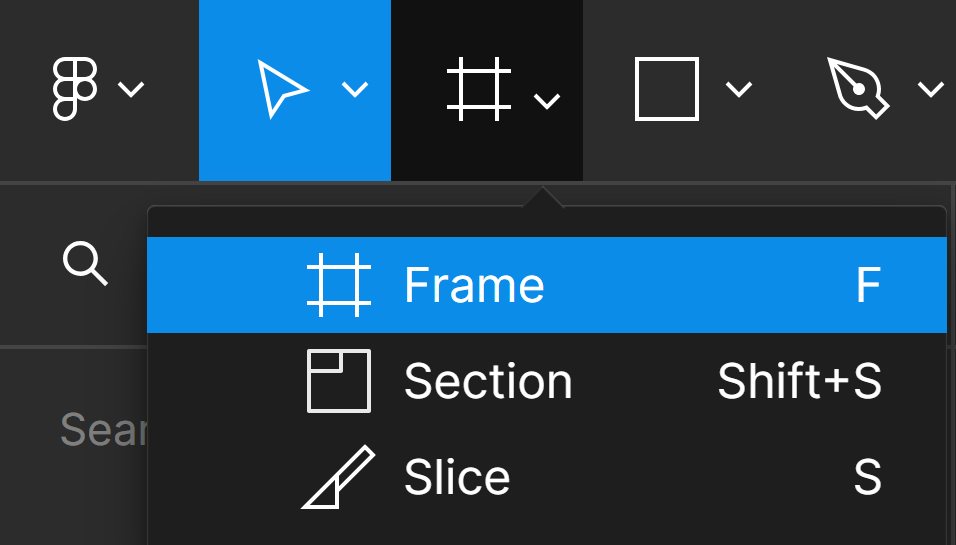
\includegraphics[width=0.5\linewidth]{imgs/img (5).png}
              \caption{Region tools}
          \end{figure}
          \newpage
    \item Shape tools: công cụ giúp tạo các hình dạng cơ bản như: Rectangle (R), Line (L), Arrow (Shift+L), Eclipse (O), Polygon, Star hoặc có thể thêm hình ảnh, video từ máy tính cá nhân thông qua "Place image/video" (Ctrl+Shift+K) 

          \begin{figure}[!h]
              \centering
              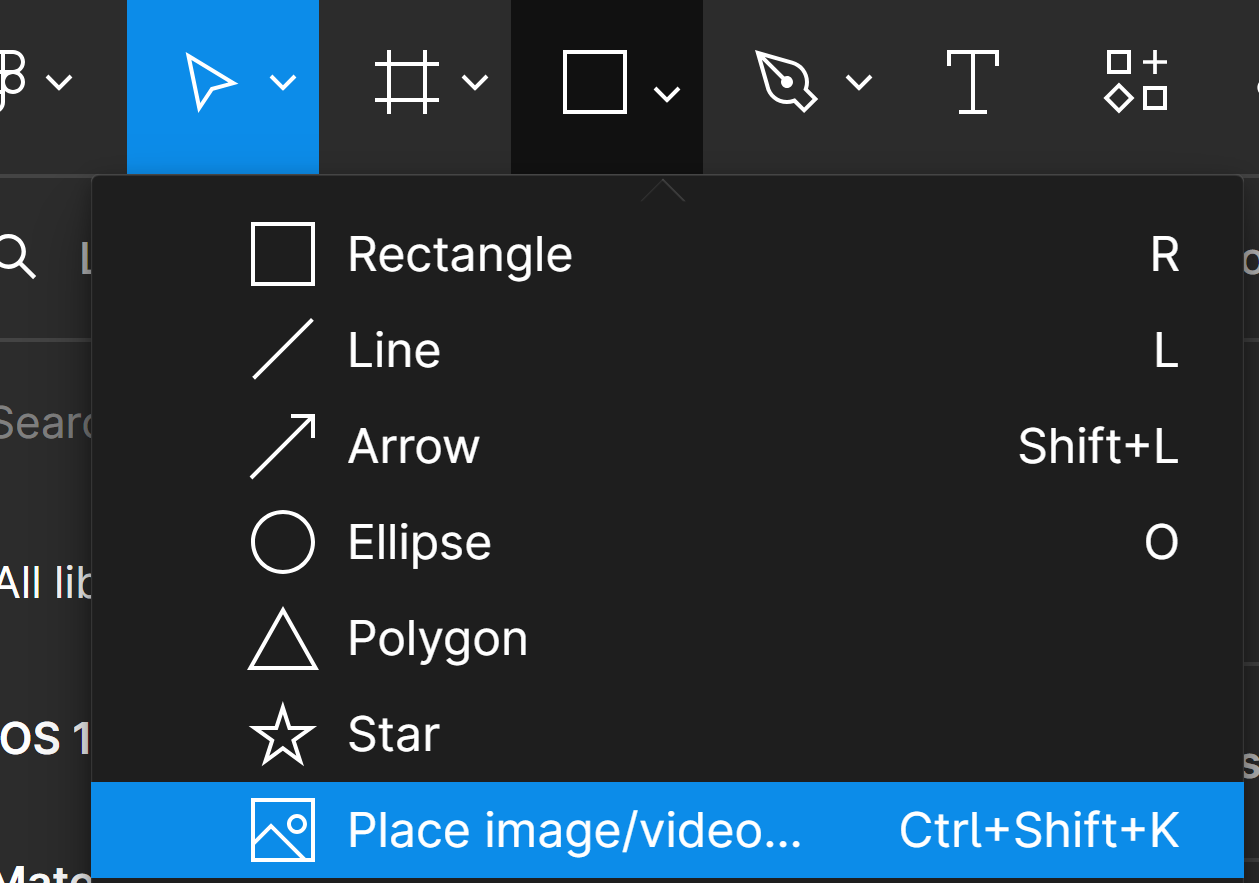
\includegraphics[width=0.5\linewidth]{imgs/img (6).png}
              \caption{Shape tools}
          \end{figure}
          \item Creation tools: công cụ giúp ta có thể vẽ hình tuỳ ý thông qua Pen (P) hay Pencil (Shift+P)

          \begin{figure}[!h]
              \centering
              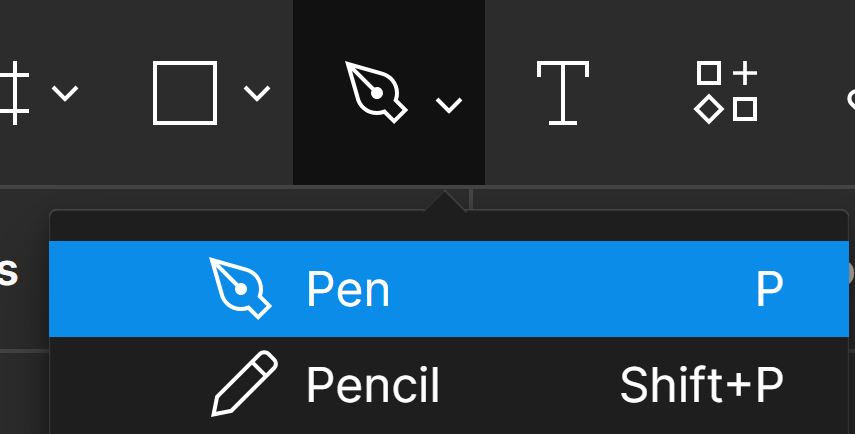
\includegraphics[width=0.5\linewidth]{imgs/img (7).png}
              \caption{Creation tools}
          \end{figure}
          \newpage
          \item Text: công cụ giúp ta thêm các đoạn văn bản vào trong bản thiết kế

          \begin{figure}[!h]
              \centering
              
\includegraphics[width=0.5\linewidth]{imgs/img (8).png}
              \caption{Text}
          \end{figure}
          \item Resources: công cụ quản lý các tài nguyên phục vụ trong thiết kế bao gồm các Components thường sử dụng, các Plugins hay Widgets đã có sẵn.

          \begin{figure}[!h]
              \centering
              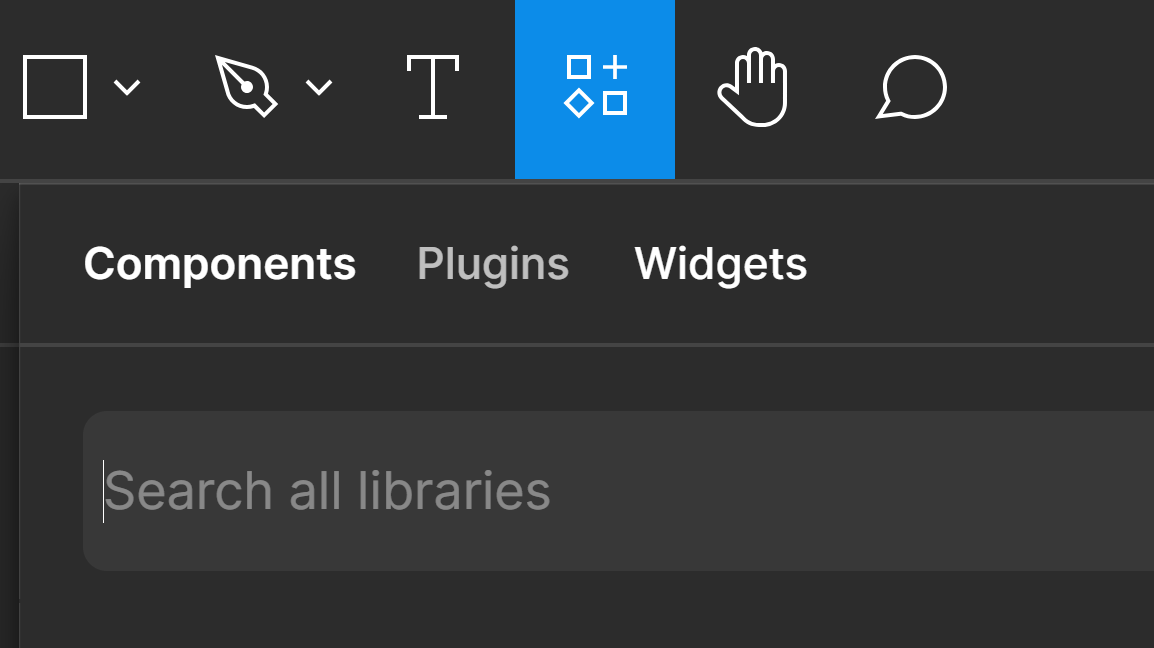
\includegraphics[width=0.5\linewidth]{imgs/img (9).png}
              \caption{Resources}
          \end{figure}
          \newpage
          \item Hand tools (H): công cụ giúp chuyển đổi góc nhìn màn hình theo ý muốn

          \begin{figure}[!h]
              \centering
              
\includegraphics[width=0.5\linewidth]{imgs/img (10).png}
              \caption{Hand tools}
          \end{figure}

    \item Cộng tác và chia sẻ
          \begin{itemize}
              \item Nhấp vào nút "Share" để tạo liên kết chia sẻ dự án với người khác.
              \item Nhấp vào nút "Collaborate" để mời người khác tham gia
              \item Thêm email để mời người khác tham gia dự án.
          \end{itemize}

\end{itemize}

\section{Các plugin nên dùng}
\begin{itemize}
    \item Anima: giúp chuyển đổi thiết kế UI/UX thành mã HTML, CSS, React và Vue một cách dễ dàng.
    \item Unsplash: Tích hợp thư viện ảnh chất lượng cao từ Unsplash vào Figma.
    \item Iconify: là một thư viện biểu tượng phong phú với hàng ngàn biểu tượng từ nhiều bộ khác nhau.
    \item Remove BG: Plugin này sử dụng công nghệ AI để xóa nền khỏi hình ảnh, giúp ta tạo ra các hình ảnh không nền nhanh chóng.
    \item Font Awesome Icons: Plugin này tích hợp các biểu tượng Font Awesome vào Figma, cho phép ta tìm kiếm và sử dụng dễ dàng.
    \item .....
\end{itemize}


\section{Kết luận}
% \item
%       \textbf{Kết luận}
Figma là một công cụ mạnh mẽ cho thiết kế giao diện người dùng và cộng tác trực tuyến. Với các chức năng đa dạng, phím tắt hữu ích, và khả năng tích hợp plugin mạnh mẽ, Figma giúp các nhà thiết kế tạo ra những sản phẩm chất lượng cao và tối ưu hóa quy trình làm việc. Hy vọng rằng tài liệu hướng dẫn này sẽ giúp ta nắm bắt và sử dụng Figma một cách hiệu quả nhất.



% \end{enumerate}

\centering{\LARGE ---------Hết---------}


\end{document}